\chapter{Experimental results}

Production delays made full-scale testing of the battery infeasible. However, the main features of the BMS have been tested separately and encouraging data has been collected.

\section{Balancing}
\begin{figure}[h]
	\centering
	\begin{tikzpicture}
    \begin{axis}[
            width=12cm,
            xmin=0, xmax=17,
            enlarge x limits=0.01,
            ylabel=Voltage,
            xlabel=Cell number,
            ybar=0,
            grid=major,
            xtick={0,...,17},
            ymin=3.79,ymax=4.0,
            use units=true,
            y unit=V, y unit prefix=m,
            every axis plot/.append style={
                    ybar,
                    bar width=1,
                    bar shift=0pt,
                    fill
                },
            legend entries={Maximum,Minimum},
            legend pos=south east
        ]
        \addplot [blue, fill=blue!60] table[x=index,y=voltage, col sep=comma, forget plot]{pictures/fenice_imbalance.csv};
        \addplot[red]coordinates{(17,3.976)};
        \addplot[yellow]coordinates{(7,3.808)};
        \addplot[blue,line legend, thick,sharp plot,nodes near coords={},
            update limits=false,shorten >=-3mm,shorten <=-3mm]
        coordinates {(0,3.908) (17,3.908)} node[above] at (8.5,3.908) {threshold};
        %\addlegendimage{line legend,black,sharp plot}

        %\node[coordinate,pin=above right:{$V_{max}$}]at (   axis cs:70,3.712)   {};
        %\node[coordinate,pin=below left:{$V_{min}$}]at (   axis cs:73,3.554)   {};
    \end{axis}
\end{tikzpicture}

	\caption{Unbalanced Fenice segment}
	\label{fig:fenice_imbalance}
\end{figure}
To test the balancing algorithm a battery pack segment was connected to a cellboard. Every pack cell was charged individually to different voltages in order to create a great imbalance. \autoref{fig:fenice_imbalance} shows the initial state of the segment with a total imbalance of $V_{17} - V_{7} = 3.976 - 3.808 = 0.168 V$. For this test the balancing settings are set to have a maximum imbalance of $100 mV$. With these settings all cells with a voltage above $V_{7} + 100 mV = 3.908 V$ need to be discharged, in this case cells 1, 3, 4, 5, 9, 10, 11, 12, 13, 14, 15, 16 and 17 are all above the threshold voltage.
The test setup only involved a single cellboard, disconnected from the mainboard. The balancing algorithm and state machine ran only on the cellboard only using its internal voltage measurements as input. A serial console was connected to a computer for monitoring and data gathering.



After starting the state machine the algorithm correctly computed the cells to balance and proceeded to the discharge state. The serial console showed the cells that were being discharged and after the predefined 30 seconds the state machine went into the cooldown state. After 10 seconds a new set of cells was computed and balancing began again.
\begin{figure}[h]
	\centering
	\begin{tikzpicture}
    \begin{axis}[
            width=12cm,
            xmin=0, xmax=17,
            enlarge x limits=0.01,
            ylabel=Voltage,
            xlabel=Cell number,
            ybar=0,
            grid=major,
            xtick={0,...,17},
            ymin=3.79,ymax=4.0,
            use units=true,
            y unit=V,
            every axis plot/.append style={
                    ybar,
                    bar width=1,
                    bar shift=0pt,
                    fill
                },
            legend entries={Minimum},
            legend pos=south east
        ]
        \addplot [blue, fill=blue!60] table[x=index,y=voltage, col sep=comma, forget plot]{pictures/fenice_balanced.csv};
        %\addplot[red]coordinates{(1,3.908)};
        \addplot[yellow]coordinates{(7,3.808)};
        \addplot[blue,line legend, thick,sharp plot,nodes near coords={},
            update limits=false,shorten >=-3mm,shorten <=-3mm]
        coordinates {(0,3.908) (17,3.908)} node[above] at (8.5,3.908) {threshold};

        %\node[coordinate,pin=above right:{$V_{max}$}]at (   axis cs:70,3.712)   {};
        %\node[coordinate,pin=below left:{$V_{min}$}]at (   axis cs:73,3.554)   {};
    \end{axis}
\end{tikzpicture}

	\caption{Fenice segment after balancing}
	\label{fig:fenice_balanced}
\end{figure}

\section{Error management}
Unit testing was used to validate the priority queue part of the system. The timer scheduling part has been tested using a logic analyzer to verify the scheduling and timing accuracy.

In \autoref{fig:error_test} the results of the test can be seen. The test scenario is analogue to the one presented in \autoref{fig:error_scheduling} in which two errors happen within the same timeframe. The two drops of channel 0 signal when the timer switches from following $E_0$ to $E_1$ and vice versa.
When the timer triggers the \texttt{Fatal} signal can be seen going high.

The timing shown in was very consistent between multiple tests, therefore the error management system can be deemed sufficiently consistent.
\begin{figure}[h]
	\centering
	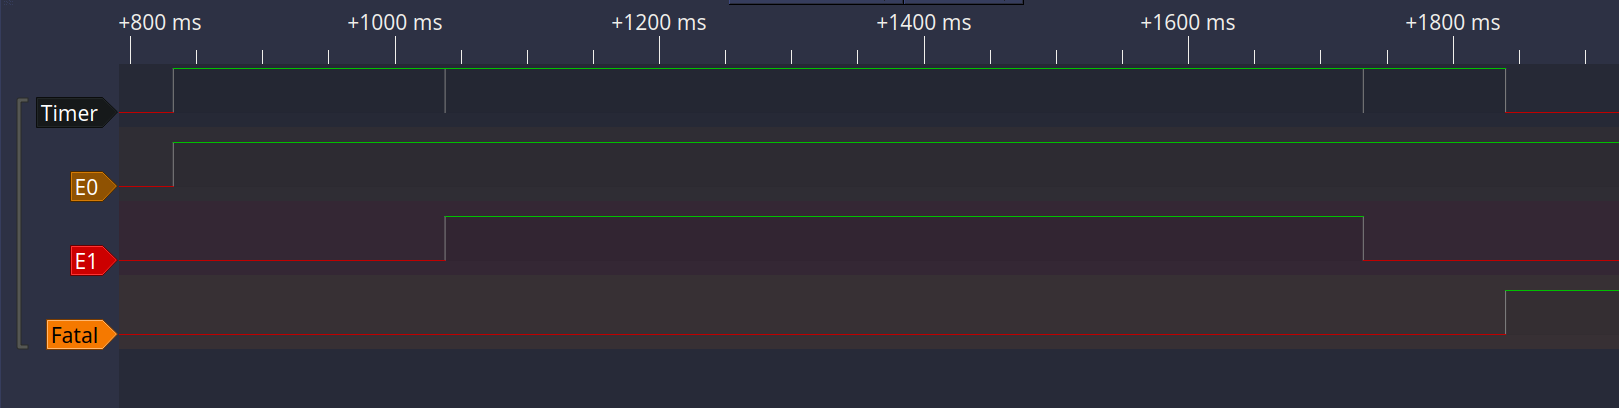
\includegraphics[width=\textwidth]{error_test}
	\caption{Error timing test.}
	\label{fig:error_test}
\end{figure}
\newpage

